\documentclass[12pt]{standalone}
\usepackage{tikz}
%\usetikzlibrary{calc, arrows.meta, decorations.pathreplacing}

\begin{document}

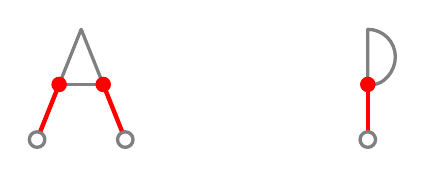
\begin{tikzpicture}[line width=1.2pt, line cap=round, line join=round, scale=1.4]
		% A
		\draw[shorten <= 2pt, shorten >= 2pt, gray] (0.2,0.5) -- (0.4,1) -- (0.6,0.5);
		\draw[shorten <= 2pt, shorten >= 2pt, gray] (0.2,0.5) -- (0.6,0.5);
		\draw[shorten >= 3.2pt, red, ultra thick] (0.2, 0.5) -- (0, 0);
		\draw[shorten >= 3.2pt, red, ultra thick] (0.6, 0.5) -- (0.8, 0);
		\fill[red] (0.2,0.5) circle(2pt);
		\fill[red] (0.6,0.5) circle(2pt);
		\draw[gray] (0,0) circle(2pt) (0.8,0) circle(2pt);

   % P
\begin{scope}[xshift=3cm]
	\draw[shorten <= 3.2pt, red, ultra thick] (0,0) -- (0,0.5); 
	\draw[shorten <= 2pt, shorten >= 2pt, gray] (0,0.5) -- (0,1) arc[start angle=90, end angle=-90, radius=0.25];
	\fill[red] (0,0.5) circle(2pt);
	\draw[gray] (0,0) circle(2pt);
	% \node[below] at (0.3,-0.2) {P};
\end{scope}
\end{tikzpicture}
\end{document}
